\newpage

\section{Simulation Analysis}
\label{sec:simulation}

In this section, we will the obtained results by simulating the circuit in Ngspice.
 
We started with by using the provided OPAMP model, and further improving by doing incremental modifications, while respecting the suitable parameters.

To decide the final best values, an optimizer was used with octave, that created a new ngspice document in each iteration as to find the suitable and most optimal values. %Escrevo isto??

The obtained values of interest can be found in table \ref{tab:sim1}.

\begin{table}[h]
    \centering
    \begin{tabular}{|l|c|}
    \hline
    {\bf Element} & {\bf Value} \\
    \hline \hline
    $Z_{input}$ & \\
    \hline
    $Z_{output}$ & \\
    \hline
    Central frequency &  Hz \\
    \hline
    Output Voltage Gain & \\
    \hline
    \end{tabular}
    \caption{Obtained values from Ngspice}
    \label{tab:sim1}
\end{table}


Using the given expression for the merit it follows that:

\begin{equation}
    Merit = 2484.9
    \label{eq:merit}
\end{equation}

Finally, below we have the plots for the frequency response.

\begin{figure}[!ht] \centering
\caption{Frequency response for the simulation analysis}
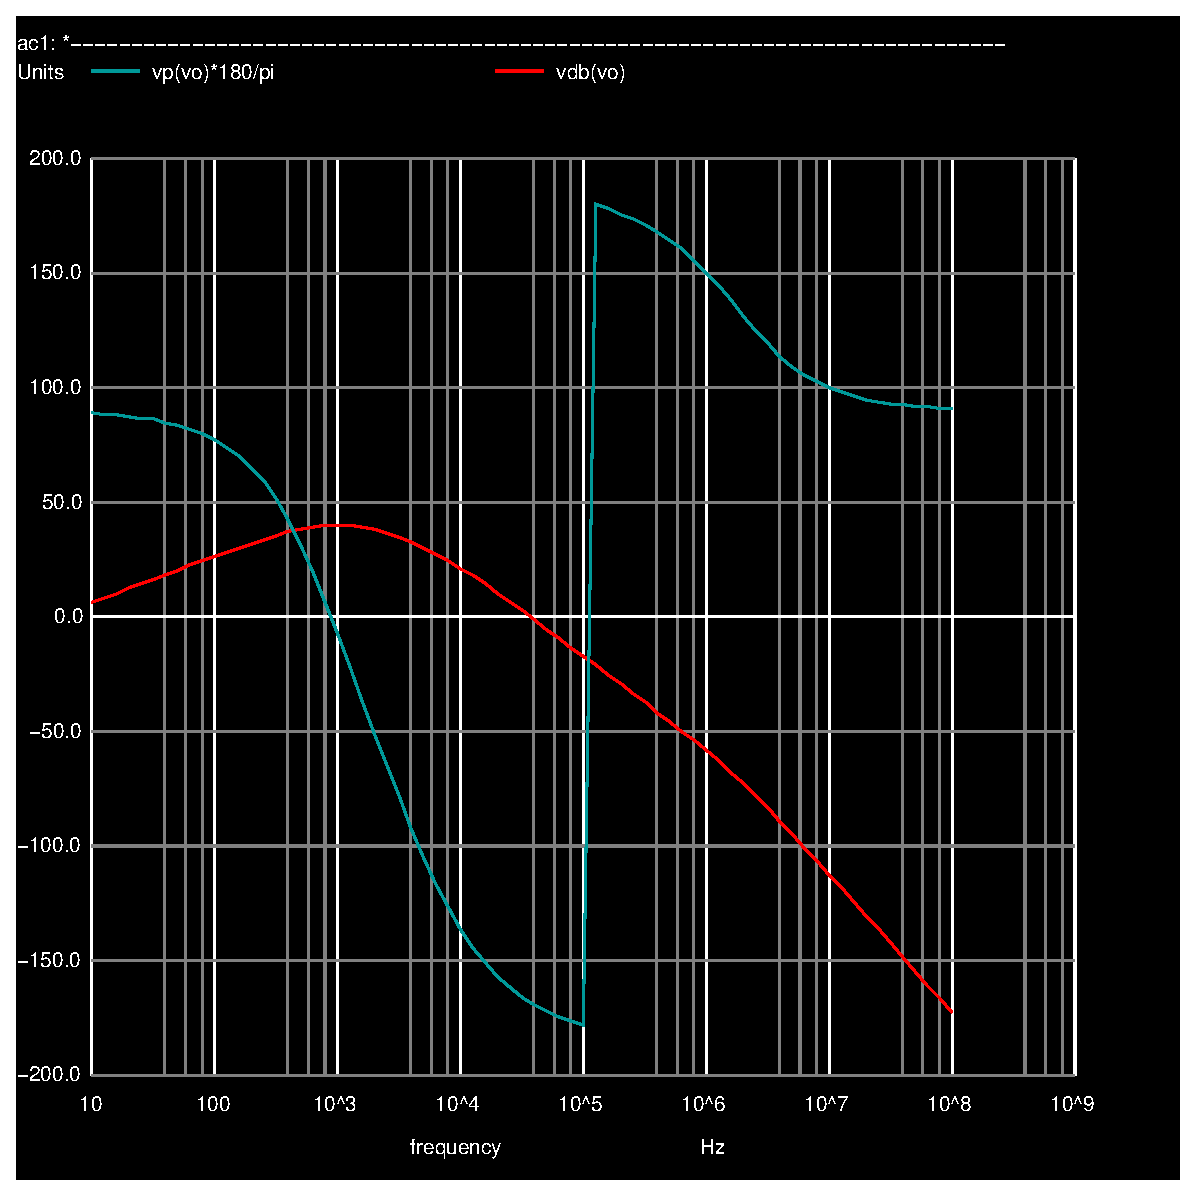
\includegraphics[width=0.8\linewidth]{simulation.eps}
\label{fig:simulation}
\end{figure}


